
C++20 added a few enhancements here and there to the existing concurrency support, but we are going to focus on the major new addition: coroutines. Coroutines, in general, are functions that can be interrupted and resumed. They are useful in several major applications: they can greatly simplify writing event-driven programs, they are almost unavoidable for work-stealing thread pools, and they make writing asynchronous I/O and other asynchronous code much easier

\subsubsubsection{8.4.1\hspace{0.2cm}The foundations of coroutines}

There are two styles of coroutines: stackful and stackless. Stackful coroutines are also sometimes called fibers; they are similar to functions wherein their state is allocated on the stack. Stackless coroutines have no corresponding stack allocations, their state is stored on the heap. In general, stackful coroutines are more powerful and flexible, but stackless coroutines are significantly more efficient.

In this book, we will focus on stackless coroutines since this is what C++20 supports. This is a sufficiently unusual concept that we need to explain before we show C++-specific syntax and examples.

A regular C++ function always has a corresponding stack frame. This stack frame exists for as long as the function is running, and that is where all the local variables and other states are stored. Here is a simple function f(): 

\begin{lstlisting}[style=styleCXX]
void f() {
	…
}
\end{lstlisting}

It has a corresponding stack frame. The function f() may call another function, g():

\begin{lstlisting}[style=styleCXX]
void g() {
	…
}
void f() {
	…
	g();
	…
}
\end{lstlisting}

The function g() also has a stack frame that exists while the function is running. 

Refer to the following figure:

\hspace*{\fill} \\ %插入空行
\begin{center}
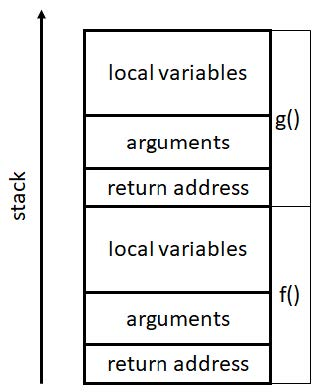
\includegraphics[width=0.9\textwidth]{content/2/chapter8/images/5.jpg}\\
Figure 8.5 – Stack frames of regular functions
\end{center}

When function g() exits, its stack frame is destroyed, and only the frame of the function f() remains.

In contrast, the state of the stackless coroutine is not stored on the stack but on the heap: this allocation is called the activation frame. The activation frame is associated with a coroutine handle, which is an object that acts as a smart pointer. Function calls can be made and returned from, but the activation frame persists as long as the handle is not destroyed. 

The coroutine also needs stack space, for example, if it calls other functions. This space is allocated on the stack of the caller. Here is how it works (the real C++ syntax is different, so think of the coroutine-related lines as pseudocode for now):

\begin{lstlisting}[style=styleCXX]
void g() {
	…
}
void coro() { // coroutine
	…
	g();
	…
}
void f() {
	…
	std::coroutine_handle<???> H; // Not the real syntax
	coro();
	…
}
\end{lstlisting}

The corresponding memory allocations are shown in the following figure:

\hspace*{\fill} \\ %插入空行
\begin{center}
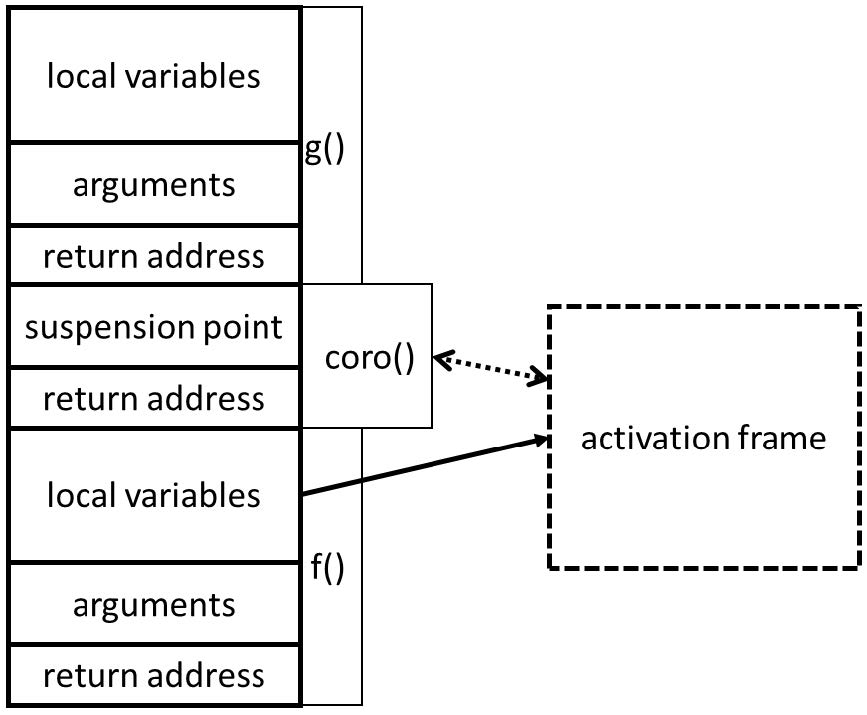
\includegraphics[width=0.9\textwidth]{content/2/chapter8/images/6.jpg}\\
Figure 8.6 – Coroutine call
\end{center}

The function f() creates a coroutine handle object, which owns the activation frame. Then it calls the coroutine function coro(). There is some stack allocation at this point, in particular, the coroutine stores on the stack the address where it would return if it is suspended (remember that coroutines are functions that can suspend themselves). The coroutine can call another function g(), which allocates the stack frame of g() on the stack. At this point, the coroutine can no longer suspend itself: it is possible to suspend only from the top level of the coroutine function. Function g() runs the same way no matter who called it and eventually returns, which destroys its stack frame. The coroutine can suspend itself now, so let us assume that it does. 

This is the key difference between stackful and stackless coroutines: a stackful coroutine can be suspended anywhere, at an arbitrary depth of function calls, and will resume from that point. But this flexibility has a high cost in memory and especially runtime: stackless coroutines, with their limited state allocations, are much more efficient.

When a coroutine suspends itself, parts of the state that are necessary to resume it are stored in the activation frame. The stack frame of the coroutine is then destroyed, and the control returns to the caller, to the point where the coroutine was called. The same happens if the coroutine runs to completion, but there is a way for the caller to find out whether the coroutine is suspended or done.

The caller continues its execution and may call other functions:

\begin{lstlisting}[style=styleCXX]
void h() {
	…
}
void coro() {…} // coroutine
void f() {
	…
	std::coroutine_handle<???> H; // Not the real syntax
	coro();
	h(); // Called after coro() is suspended
	…
}
\end{lstlisting}

The memory allocations now look as follows:

\hspace*{\fill} \\ %插入空行
\begin{center}
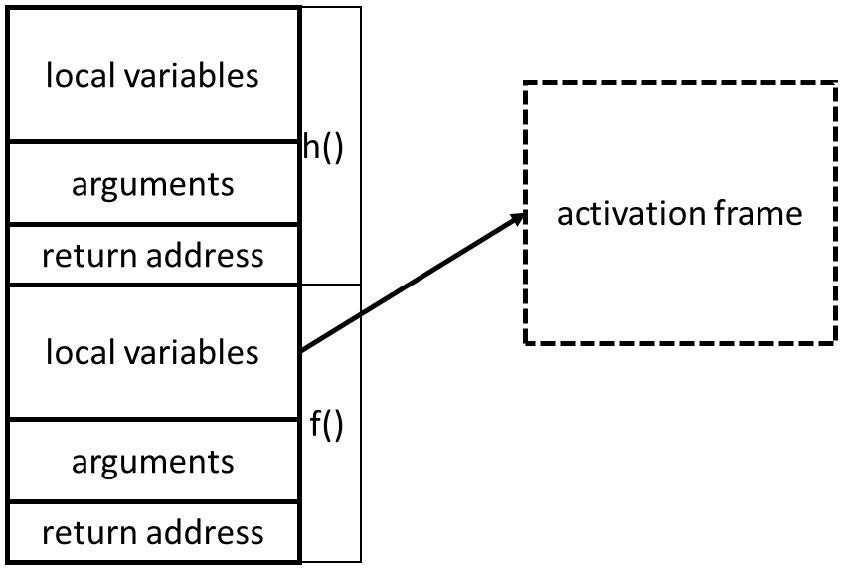
\includegraphics[width=0.9\textwidth]{content/2/chapter8/images/7.jpg}\\
Figure 8.7 – Coroutine is suspended, execution continues
\end{center}

Note that there is no stack frame corresponding to the coroutine, only the heap-allocated activation frame. The coroutine can be resumed as long as the handle object is alive. It does not have to be the same function that calls and resumes the coroutine; for example,  our function h() can resume it if it has access to the handle:

\begin{lstlisting}[style=styleCXX]
void h(H) {
	H.resume(); // Not the real syntax
}
void coro() {…} // coroutine
void f() {
	…
	std::coroutine_handle<???> H; // Not the real syntax
	coro();
	 h(H); // Called after coro() is suspended
	…
}
\end{lstlisting}

The coroutine resumes from the point where it was suspended. Its state is restored from  the activation frame, and any necessary stack allocations will happen as usual:

\hspace*{\fill} \\ %插入空行
\begin{center}
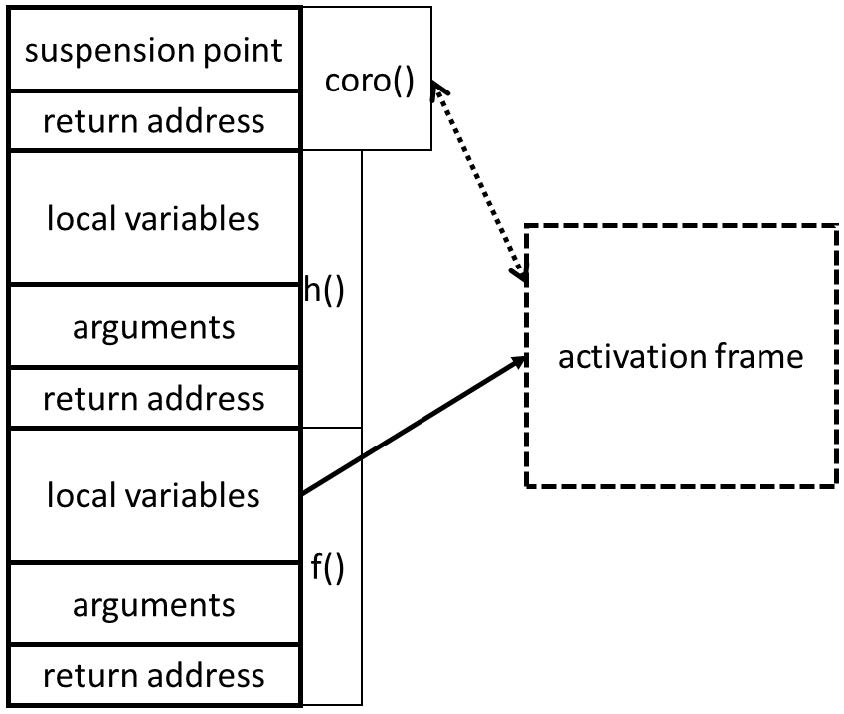
\includegraphics[width=0.9\textwidth]{content/2/chapter8/images/8.jpg}\\
Figure 8.8 – Coroutine is resumed from a different function
\end{center}.

Eventually, the coroutine completes, and the handle is destroyed; this deallocates all the memory associated with the coroutine.

Here is a summary of what is important to know about C++20 coroutines:

\begin{itemize}
\item
Coroutines are functions that can suspend themselves. This is different from the OS suspending a thread: suspending a coroutine is done explicitly by the programmer (cooperative multitasking).

\item
Unlike regular functions, which are associated with stack frames, coroutines have handle objects. Coroutine state persists as long as the handle is alive.

\item
After the coroutine is suspended, the control is returned to the caller, which continues to run the same way as if the coroutine had completed. 


\item 
The coroutine can be resumed from any location; it does not have to be the caller itself. Furthermore, the coroutine can even be resumed from a different thread (we will see an example later in this section). The coroutine is resumed from the point of suspension and continues to run as if nothing happened (but may be running on a different thread).
\end{itemize}

Now let us see how all of this is done in real C++.

\subsubsubsection{8.4.2\hspace{0.2cm}Coroutine C++ syntax}

Let us now see the C++ language constructs that are used for programming with coroutines. 

The first order of business is getting a compiler that supports this feature. Both GCC and Clang have coroutine support in their latest versions, but, unfortunately, not in the same way. For GCC, you need version 11 or later. For Clang, partial support was added in version 10 and was improved in later versions, although it still remains "experimental."

First of all, in order to compile coroutine code, you need a compiler option on the command line (merely enabling C++20 with the --std=c++20 option is not enough). For GCC, the option is –fcoroutines. For Clang, the options are -stdlib=libc++ -fcoroutines-ts. No options except /std:c++20 are needed for the latest Visual Studio.

Then, you need to include the coroutines header. In GCC and Visual Studio (and according to the standard), the header is \#include <coroutine> and all the classes it declares are in namespace std. Unfortunately, in Clang, the header is \#include <experimental/coroutine> and the namespace is std::experimental. 

There is no special syntax for declaring a coroutine: coroutines are, syntactically, just regular C++ functions. What makes them into coroutines is the use of the suspend operator co\_await or its variant, co\_yield. However, it's not enough to call one of these operators in the body of the function: coroutines in C++ have strict requirements for their return types. The standard library offers no help in declaring these return types and other classes necessary for working with coroutines. The language provides only a framework for programming with coroutines. As a result, the coroutine code that uses C++20 constructs directly is very verbose, repetitive, and contains a lot of boilerplate code. In practice, everybody who uses coroutines does so using one of several available coroutine libraries. 

For practical programming, so should you. However, in this book, we show you examples written in bare C++. We do it because we do not want to direct you toward any particular library and because doing so would obscure the understanding of what is really going on. The support for coroutines is very recent, and the libraries are rapidly evolving; it is unlikely that your library of choice will stay the same. We would like you to understand the coroutine code at the C++ level instead of at the level of abstractions presented by a particular library. Then you should choose a library based on your needs and use its abstractions.

A thorough description of the syntax constructs related to coroutines would be 
remarkably non-intuitive: it is a framework, not a library. For that reason, we do the rest of the presentation using examples. If you really want to know all the syntax requirements for coroutines, you have to look up a very recent publication (or read the standard). But the examples should give you enough understanding of what coroutines can do that you can read the documentation for your favorite coroutine library instead and use it in your  programs.

\subsubsubsection{8.4.3\hspace{0.2cm}Coroutine examples}

The first example is probably the most common use of coroutines in C++ (and the one for which the standard provides some explicitly designed syntax). We are going to implement a lazy generator. Generators are functions that generate sequences of data; every time you call the generator, you get a new element of the sequence. A lazy generator is a generator that computes elements on demand, as it is called. 

Here is a lazy generator based on C++20 coroutines:

\hspace*{\fill} \\ %插入空行
\noindent
\textbf{coroutines\_generator1.C}
\begin{lstlisting}[style=styleCXX]
generator<int> coro(){
	for (int i = 0;; ++i) {
		co_yield i;
	}
}
int main() {
	auto h = coro().h_;
	auto& promise = h.promise();
	for (int i = 0; i < 3; ++i) {
		std::cout << "counter: " << promise.value_ << 
		std::endl;
		h();
	}
	h.destroy();
}
\end{lstlisting}

As promised, this is very low-level C++, you rarely see code like this, but it allows us to explain all the steps. First of all, the coroutine coro() looks like any other function, except for the co\_yield operator. This operator suspends the coroutine and returns the value i to the caller. Because the coroutine is suspended, not terminated, the operator can be executed multiple times. Just like any other function, the coroutine terminates when the control reaches the closing brace; at this point, it cannot be resumed. It is possible to exit the coroutine at any point by executing statement co\_return (the regular return statement should not be used).

Second, the return type of the coroutine – generator – is a special type that we are about to define. It has a lot of requirements on it, which results in lengthy boilerplate code (any coroutine library will have such types predefined for you). We can already see that generator contains a nested data member h\_; that is the coroutine handle. The creation of this handle also creates the activation frame. The handle is associated with a promiseobject; this has absolutely nothing to do with C++11 std::promise. In fact, it is not one of the standard types at all: we have to define it according to a set of rules listed in the standard. At the end of the execution, the handle is destroyed, which destroys the coroutine state as well. The handle is, thus, similar to a pointer.

Finally, the handle is a callable object. Calling it resumes the coroutine, which generates the next value and promptly suspends itself again because the co\_yield operator is in the loop. 

All of this is magically tied together by defining the appropriate return type for the coroutine. Just like the STL algorithms, the entire system is bound by convention: there are expectations on all types involved in this process, and something somewhere will not compile if these expectations are not met. Let us see the generator type now:

\begin{lstlisting}[style=styleCXX]
template <typename T> struct generator {
	struct promise_type {
		T value_ = -1;
		generator get_return_object() {
			using handle= std::coroutine_handle<promise_type>;
			return generator{handle::from_promise(*this)};
		}
		std::suspend_never initial_suspend() { return {}; }
		std::suspend_never final_suspend() noexcept { return 
			{}; }
		void unhandled_exception() {}
		std::suspend_always yield_value(T value) {
			value_ = value;
			return {};
		}
	};
	std::coroutine_handle<promise_type> h_;
};
\end{lstlisting}

First of all, the return type does not have to be generated from a template. We could have just declared a generator for integers. Usually, it is a template parameterized on the type of the elements in the generated sequence. Second, the name generator is in no way special: you can call this type anything you want (most libraries provide a similar template and call it generator). On the other hand, the nested type generator::promise\_type must be called promise\_type, otherwise, the program will not compile. Often,  the nested type itself is called something else, and a type alias is used:

\begin{lstlisting}[style=styleCXX]
template <typename T> struct generator {
	struct promise { … };
	using promise_type = promise;
};
\end{lstlisting}

The promise\_type type must be a nested type of the generator class (or, in general, any type returned by the coroutine). But the promise class does not have to be a nested class: usually, it is, but it could be declared outside as well. 

What is mandatory is the set of required member functions of the promise type, including their signatures. Note that some of the member functions are declared noexcept. This is part of the requirement, too: the program will not compile if you omit this specification. Of course, any function that is not required to be noexcept can be declared as such if it doesn't throw. 

The body of these required functions may be more complex for different generators. We will describe briefly what each of them does.

The first non-empty function, get\_return\_object(), is part of the boilerplate code and usually looks exactly like the one earlier; this function constructs a new generator from a handle that is, in turn, constructed from a promise object. It is called by the compiler to get the result of the coroutine. 

The second non-empty function, yield\_value(), is invoked every time the operator co\_yield is called; its argument is the co\_yield value. Storing the value in the promise object is how the coroutine usually passes the results to the caller. 

The initial\_suspend() function is called by the compiler the first time co\_yield is encountered. The final\_suspend() function is called after the coroutine produces its last result via co\_return; it cannot be suspended afterward. If the coroutine ends without co\_return, the return\_void() method is called. Finally, if the coroutine throws an exception that escapes from its body, the unhandled\_exception() method is called. You can customize these methods for special handling of each of these situations, although this is seldom used.

Now we see how it all ties together to provide us with a lazy generator. First, the coroutine handle is created. In our example, we do not keep the generator object, only the handle. This is not required: we could have kept the generator object and destroyed the handle in its destructor. The coroutine runs until it hits co\_yield and suspends itself; the control is returned by the caller while the return value of co\_yield is captured in the promise. The calling program retrieves this value and resumes the coroutine by invoking the handle. The coroutine picks up from the point where it was suspended and runs until the next co\_yield. 

Our generator can run forever (or until we reach the maximum integer value on our platform, anyway): the sequence never ends. If we needed a sequence of finite length, we can execute co\_return or just exit the loop after the sequence is over. Refer to the following code:

\begin{lstlisting}[style=styleCXX]
generator<int> coro(){
	for (int i = 0; i < 10; ++i) {
		co_yield i;
	}
}
\end{lstlisting}

Now we have a sequence of 10 elements. The caller must check the result of the handle member function done() before trying to resume the coroutine.

We mentioned before that a coroutine can be resumed from anywhere in the code (after it was suspended, of course). It can even be resumed from a different thread. In this case, the coroutine starts to execute on one thread, is suspended, and then runs the rest of its code on another thread. Let us see an example:

\hspace*{\fill} \\ %插入空行
\noindent
\textbf{coroutines\_change\_threads.C}
\begin{lstlisting}[style=styleCXX]
task coro(std::jthread& t) {
	std::cout << "Coroutine started on thread: " <<
		std::this_thread::get_id() << '\n';
	co_await awaitable{t};
    std::cout << "Coroutine resumed on thread: " <<
		std::this_thread::get_id() << '\n';
	std::cout << "Coroutine done on thread: " <<
		std::this_thread::get_id() << '\n';
}
int main() {
	std::cout << "Main thread: " <<
		std::this_thread::get_id() << '\n';
	std::jthread t;
	coro(t);
	std::cout << "Main thread done: " << 
		std::this_thread::get_id() << std::endl;
}
\end{lstlisting}

First, let us get one detail out of the way: std::jthread is a C++20 addition, it is just a joinable thread – it is joined in the destructor of the object (almost anyone who worked with threads wrote a class for that, but now we have a standard one). Now we can move to the important part – the coroutine itself. 

First, let us see the return type of the coroutine:

\begin{lstlisting}[style=styleCXX]
struct task{
	struct promise_type {
		task get_return_object() { return {}; }
		std::suspend_never initial_suspend() { return {}; }
		std::suspend_never final_suspend() noexcept { return 
			{}; }
		void return_void() {}
		void unhandled_exception() {}
	};
};
\end{lstlisting}

This is actually the smallest possible return type of a coroutine: it contains all the required boilerplate and nothing else. Specifically, the return type is a class that defines a nested type promise\_type. That nested type must define several member functions, as shown in this code. Our generator type from the previous example has all of that plus some data used to return the results to the caller. Of course, the task can also have an internal state as needed.

The second change from the previous example is the way the task is suspended: we do it with co\_await instead of co\_yield. Operator co\_await is actually the most general way to suspend a coroutine: just like co\_yield, it suspends the function and returns the control to the caller. The difference is in the argument type: while co\_yield returns a result, co\_await's argument is an awaiter object with very general functionality. There are, again, specific requirements on the type of this object. If the requirements are met, the class is called an awaitable, and an object of this type is a valid awaiter (if not, something somewhere will not compile). Here is our awaitable:

\begin{lstlisting}[style=styleCXX]
struct awaitable {
	std::jthread& t;
	bool await_ready() { return false; }
	void await_suspend(std::coroutine_handle<> h) {
		std::jthread& out = t;
		out = std::jthread([h] { h.resume(); });
	}
	void await_resume() {}
	~awaitable() {}
	awaitable(std::jthread& t) : t(t) {}
};
\end{lstlisting}

The required interface of an awaitable is the three methods we see here. The first is await\_ready(): it is called after the coroutine is suspended. If it returns true, then the result of the coroutine is ready, and it is not really necessary to suspend it. In practice, it almost always returns false, which leads to suspension of the coroutine: the state of the coroutine, such as local variables and the suspension point, is stored in the activation frame, and the control is returned to the caller or resumer. The second function is await\_resume(), it is called just before the coroutine continues to execute after it is resumed. If it returns the result, that is the result of the entire co\_await operator (no result in our example). The most interesting function is await\_suspend(). It is called with the handle of the current coroutine when this coroutine is suspended and can have several different return types and values. If it returns void, as it does in our example, the coroutine is suspended, and the control is returned to the caller or resumer. Don't be fooled by the content of await\_suspend() in our example: it does not resume the coroutine. Instead, it creates a new thread that will execute a callable object, and it is this object that resumes the coroutine. The coroutine may be resumed after await\_suspend() is done or while it is still running: this example demonstrates the use of coroutines for asynchronous operations. 

Putting all of this together, we get this sequence:

\begin{enumerate}
\item
The main thread calls a coroutine.

\item
The coroutine is suspended by operator co\_await. This process involves several calls to the member functions of the awaitable object, one of which creates a new thread whose payload resumes the coroutine (the game with move-assigning thread objects is done so we delete the new thread in the main program and avoid some nasty race conditions).

\item
Control is returned to the caller of the coroutine, so the main thread continues to run from the line after the coroutine call. It will block in the destructor of the thread object t if it gets there before the coroutine completes.

\item 
The coroutine is resumed by the new thread and continues to execute on that thread from the line after co\_await. The awaitable object that was constructed by co\_await is destroyed. The coroutine runs to the end, all on the second thread. Reaching the end of the coroutine means it's done, just like any other function. The thread that runs the coroutine now can be joined. If the main thread was waiting for the destructor of thread t to complete, it now unblocks and joins the thread (if the main thread has not yet reached the destructor, it won't block when it does). 
\end{enumerate}

The sequence is confirmed by the output of our program:

\begin{tcblisting}{commandshell={}}
Main thread: 140003570591552
Coroutine started on thread: 140003570591552
Main thread done: 140003570591552
Coroutine resumed on thread: 140003570587392
Coroutine done on thread: 140003570587392
\end{tcblisting}

As you can see, the coroutine coro() was running on one thread first, then changed to a different thread in the middle of the execution. If it had any local variables, they would be preserved through this transition.

We mentioned that co\_await is the general operator for suspending coroutines. Indeed, the co\_yield x operator is equivalent to a particular invocation of co\_await as shown here:

\begin{lstlisting}[style=styleCXX]
co_await promise.yield_value(x);
\end{lstlisting}

Here promise is the promise\_type object associated with the current coroutine handle. The reason for the separate operator co\_yield is that accessing your own promise from inside the coroutine results in a quite verbose syntax, so the standard added a shortcut.

These examples demonstrate the capabilities of coroutines in C++. The situations where coroutines are thought to be useful are work stealing (you have seen how easy it is to transfer execution of a coroutine to another thread), lazy generators, and asynchronous operations (I/O and event handling). Nonetheless, the C++ coroutines have not been around long enough for any patterns to emerge, so the community is yet to come up with the best practices for using coroutines. Similarly, it is too early to talk about the performance of the coroutines; we have to wait for the compiler support to mature and for larger-scale applications to be developed. 

Overall, after neglecting concurrency for years, the C++ standard is rapidly catching up, so let us summarise the recent advances.









